\section*{Nadaljevanje: NVILA-8B in Florence-2-large na RTX 5090}
Nova primerjava uporablja istih 100 RGB slik in isti razpršeni podnabor 20 slik. Referenčne vrste in okvirji niso vhod modelov. Prejšnjih uspešnih inferenc Qwen/Gemma ne ponavljamo; v tabelah uporabimo njihove shranjene izhode 2. dela. Rezultati so povezani pogledi dveh prostorov.
\subsection*{Dejanski izolirani zagon in razlike nalog}
Oba nova modela sta bila zagnana v ločenih Docker okoljih: Python 3.11, PyTorch 2.7.1+cu128, CUDA 12.8, Transformers 4.46.0. Binarne datoteke vsebujejo sm\_120; vsak parameter je preverjeno na GPU. NVILA ima 8,09 milijarde parametrov, Florence približno 0,776 milijarde. Oba dejansko računata v FP16; to ni Qwenova BF16 referenca ali kvantizacija Q4.

NVILA uporablja uradno VILA kodo, pripeto na 57ecbfb904b9, in originalne uteži NVILA-8B. Neposredni izvajalnik odstrani omejitev starega API seznama dovoljenih modelov. Python gostitelja se ne uporablja. Starega torch 2.3/CUDA 12.2 FlashAttention ne namestimo: Qwen2 in SigLIP uporabita SDPA. Učne/FP8 uvoze in neuporabljene vizualne arhitekture izločimo; dinamični S2 ter projektor in uteži ostanejo. Natančen popravek in vse napake so shranjeni. Model ni preimenovan v 15B.

NVILA prejme isti rich-v2 prompt in slikovne bajte kot 2. del, greedy T=0, seed 42, največ 8192 izhodnih tokenov in kontekst 16384. Top-p/top-k sta pri greedy neaktivna. Kazen prisotnosti iz Ollame ni podprta; ločeno uporabimo repetition\_penalty=1,05 iz konfiguracije NVILA uteži. Začetni diagnostični pilot z ovojevo vrednostjo 1,0 je dosegel limit in ponavljal zapise; ohranjen je ločeno, brez tihega popravka.

Florence prejme samo tri izvirne kontrolne tokene: \texttt{<MORE\_DETAILED\_CAPTION>}, \texttt{<OD>}, \texttt{<DENSE\_REGION\_CAPTION>}. Ne dobi Qwenovega prompta ali sheme. Uporabimo zahtevani osnovni \texttt{microsoft/Florence-2-large}, ne različice \texttt{-ft}. Nastavitve so največ 1024 tokenov, num\_beams=3, do\_sample=false, seed 42; pozornost eager. Njegov predprocesor in ločljivost se razlikujeta od dinamičnega S2 in Ollame. Razlike modelov, števila parametrov, dolžin in nalog preprečujejo arhitekturno ali vzročno razlago hitrosti.
\subsection*{Časi vseh odgovorov, tudi zavrnjenih; brez ogrevanja}
\begin{center}\small\begin{tabular}{p{3.4cm}p{3.1cm}rrrr}\toprule
Model & Naloga & Velj./vsi & Povp. s & Med. s & p90 s \\ \midrule
NVILA-8B FP16 & rich & 0/100 & 29.18 & 9.26 & 133.73 \\
Florence-2-large FP16 & caption & 100/100 & 0.42 & 0.42 & 0.50 \\
Florence-2-large FP16 & od & 100/100 & 0.19 & 0.14 & 0.38 \\
Florence-2-large FP16 & dense & 99/100 & 0.34 & 0.23 & 0.61 \\
Florence-2-large FP16 & combined & 99/100 & 0.95 & 0.83 & 1.42 \\
Qwen BF16 (staro) & rich-v2 & 69/100 & 13.25 & 11.52 & 19.00 \\
Qwen Q4 (staro) & rich-v2 & 82/100 & 5.13 & 4.09 & 6.06 \\
Gemma Q4 (staro) & rich-v2 & 89/100 & 4.23 & 4.15 & 5.29 \\
\bottomrule\end{tabular}\end{center}

Florence combined je neposredno merjen celotni postopek treh zaporednih nalog na sliko, s predprocesiranjem, razčlenjevanjem in zapisi JSON; izris slik je izključen. To ni samo čas ene od nalog. Skupni merjeni čas kombiniranega postopka za 100 slik je 94.97 s. Surovi tokeni in ID-ji so ohranjeni. Števila tokenov različnih tokenizerjev niso neposredno primerljiva. Veljaven zapis ne pomeni pravilnega opisa.

\newpage
\section*{Pomnilnik, lokalizacija in besedilna presoja}
\begin{center}\small\begin{tabular}{p{4cm}p{3.8cm}rrr}\toprule
Model & Dejanski tipi & Alloc. GiB & Reserv. GiB & Nalag. s \\ \midrule
NVILA-8B FP16 & torch.float16 & 16.50 & 19.55 & 30.18 \\
Florence-2-large FP16 & torch.float16 & 1.98 & 2.12 & 0.69 \\
\bottomrule\end{tabular}\end{center}

Allocated/reserved sta procesna vrhova PyTorch, ne isti podatek kot Ollama size\_vram. Skupna poraba iz nvidia-smi vključuje namizje in tuje procese; surovi časovni vzorci so shranjeni. Nalaganje je ločeno; tabela kaže zadnjo sejo. Fizično ogrevanje po vsakem nalaganju je izključeno iz glavnih 100 slik: NVILA-8B FP16: 2 klicev, skupaj 9.1 s; Florence-2-large FP16: 9 klicev, skupaj 2.9 s. Začetna diagnostika NVILA je dodatna in ločena. Shranjeni prvi merjeni odgovori se ob nadaljevanju ponovno uporabijo.
\subsection*{Okvirji: dokumentirano ujemanje z anotiranimi regijami}
Florence napove xyxy v pikah izvirne slike. Validator preveri končnost, vrstni red in meje; okvirjev ne obrezuje ali popravlja. Izrisanih je do 200 slik (OD in dense za vsako sliko). Ujemanje je po isti sliki/SHA256 in vnaprej določenem slovarju imen (npr. person/people/man/woman $\rightarrow$ People); brez podnizov ali samodejnega ugibanja samostalnika v dolgi frazi. Pri IoU $\geq 0,5$ uporabimo največje enolično dvodelno ujemanje. Vsak par, imeni in oba okvirja so v extended-box-matches.json; slovar, izključitve in algoritem so v Git.
\begin{center}\small\begin{tabular}{p{2.1cm}p{1.5cm}rrrr}\toprule
Nabor & Naloga & Nap. regije & Mapirana imena & Ujem./ref. & Povp. IoU \\ \midrule
trgovina & od & 147 & 65 & 39/495 & 0.88 \\
trgovina & dense & 210 & 70 & 10/495 & 0.81 \\
agtea & od & 750 & 634 & 303/963 & 0.82 \\
agtea & dense & 793 & 469 & 188/963 & 0.81 \\
\bottomrule\end{tabular}\end{center}

To je pokritost anotiranih regij v omejenem slovarju, ne popolna natančnost detekcije. Products/Fruits in druge vrste zunaj slovarja so izključene; skupinska oznaka ne pomeni ene instance. Nepovezana napoved ni avtomatično halucinacija, ker reference niso izčrpne. Dolga dense fraza lahko pravilno opiše regijo, a nima dobesednega razrednega ujemanja. Zato ne poročamo mAP, skupnega precision/recall/F1 ali caption accuracy. Qwen/Gemma in NVILA v tej primerjavi nimajo napovedanih okvirjev; prostorskega besedila ne pretvorimo v IoU.
\subsection*{Drugi korak: isti Qwen BF16 na istih 20 slikah}
NVILA veljavni rich opisi ostanejo v celoti nespremenjeni. Pri zavrnjenem rich izhodu ločen transport literal-native-text-v1 ohrani celoten surovi odgovor kot sceno, iz prvega strogo razčlenjenega JSON predponskega objekta pa vzame samo dobesedna imena in celotne izvirne objekte kot opazovanja. Izvirni odgovor ostane zavrnjen, ne postane veljaven rich JSON; nič besedila se ne zavrže. Če ni takega seznama ali so ključi podvojeni, je preskok. To je ločen besedilni preizkus, ne primerjava popolnoma iste vstopne sheme.

Florencejev opis ter OD oznake in dense fraze pretvorimo dobesedno: vsaka izvirna regija dobi lokalni ID in izvirno oznako/frazo ter okvir v besedilu. Regij med nalogama ne združujemo kot isto instanco. Ne dodamo materialov, stikov, namestitev ali odnosov. Transportni not\_visible pomeni nepodan/neveljaven dokaz namestitve; identifiable=true označi modelovo imenovano regijo, ne ročne potrditve. NVILA izvirne veljavne oznake dokazov ohranimo; ostale izvirne trditve ostanejo v opazovanju kot modelove trditve. Izhodi in izvorni SHA so zamrznjeni; drugi korak ne bere ali pošilja slik.
\begin{center}\small\begin{tabular}{p{3cm}p{4cm}rrr}\toprule
Opisovalnik & OK/napaka/preskok & fixed & movable & uncertain \\ \midrule
nvila & 14/2/4 & 26 & 22 & 13 \\
florence & 20/0/0 & 52 & 216 & 98 \\
\bottomrule\end{tabular}\end{center}

Razvrščanje uporabi prejšnji short-no-examples prompt, T=0,3, seed 42. Opisi brez veljavnega dobesednega prenosa ostanejo preskočeni; napake razvrščanja niso popravljene. nvila: 16 merjenih klicev, povprečje 2.04 s, največ 8857 vhodnih tokenov; florence: 20 merjenih klicev, povprečje 3.59 s, največ 9913 vhodnih tokenov. Vseh 36 merjenih klicev in štiri izključena ogrevanja imajo potrjen GPU; kontekst je 16384. Različna granularnost regij pomeni, da števila razredov niso accuracy ali strinjanje istih instanc. Referenc stabilnosti ni; razlogi so modelove trditve, ne potrditev dejanskega pritrjevanja.

\newpage
\section*{Dejanski primeri: fotografija in Florence regije}\subsection*{Trgovina / indeks 1}
\begin{center}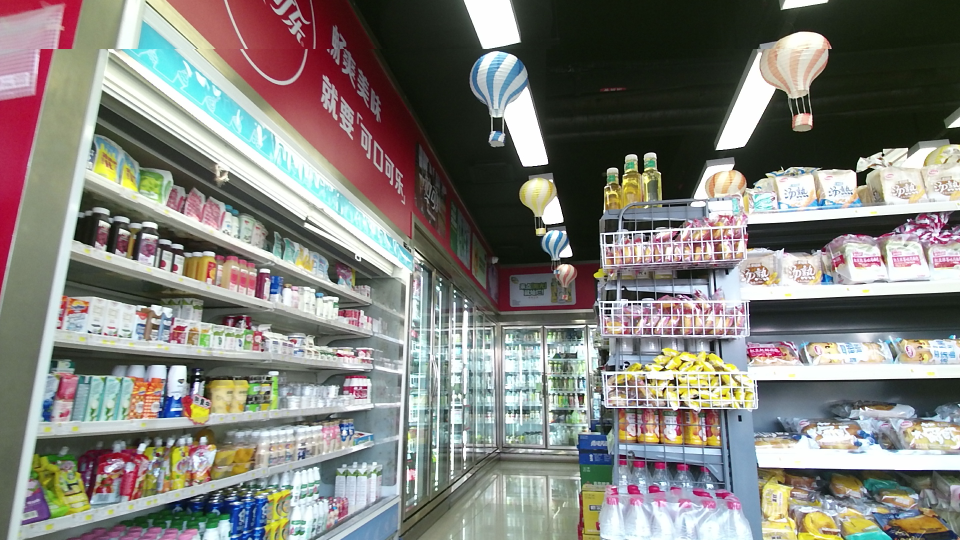
\includegraphics[width=.32\linewidth]{figures/extended-thud_dense_test50-1-rgb.png}\hfill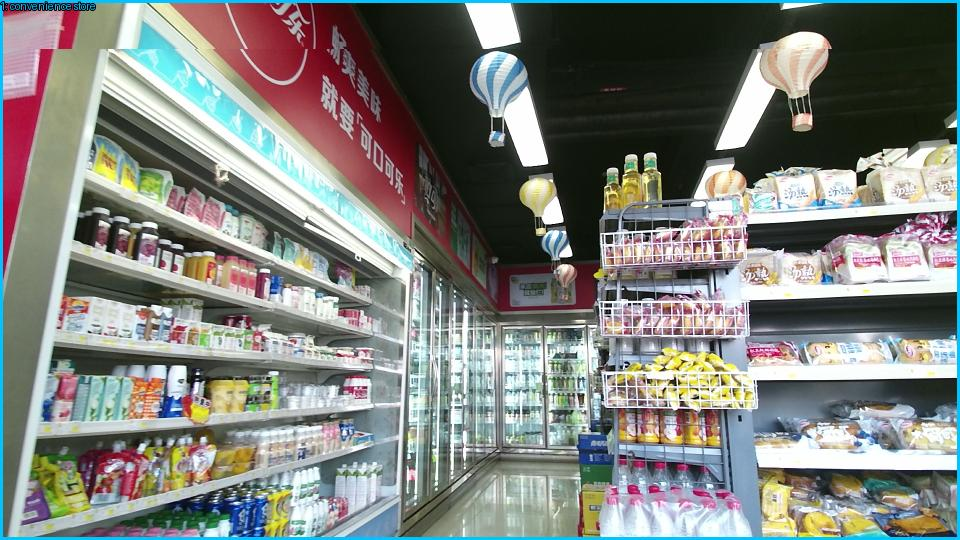
\includegraphics[width=.32\linewidth]{figures/extended-thud_dense_test50-1-od.jpg}\hfill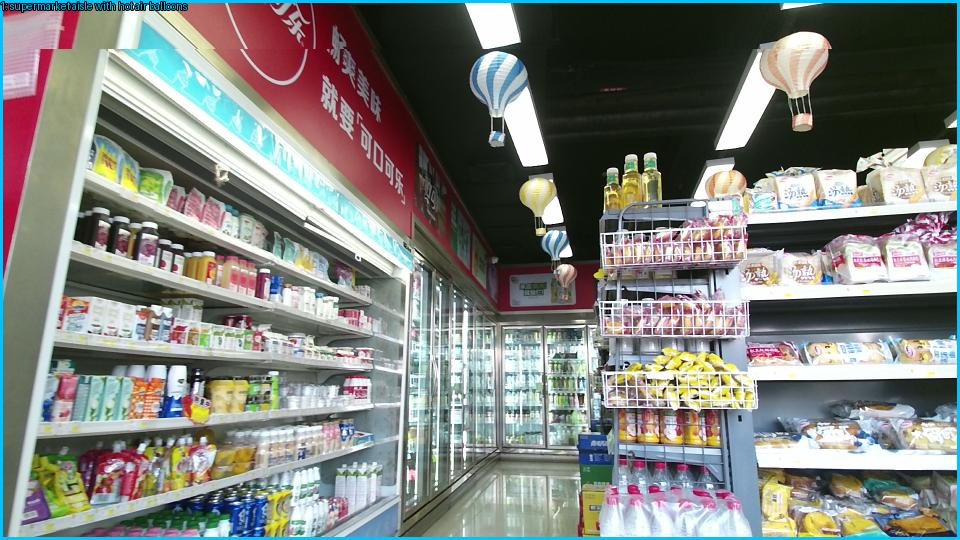
\includegraphics[width=.32\linewidth]{figures/extended-thud_dense_test50-1-dense.jpg}\\{\scriptsize Levo: RGB; sredina: OD; desno: DENSE\_REGION\_CAPTION. Okvirji so napovedi, ne reference.}\end{center}
\begin{center}\small\begin{tabular}{p{3.2cm}p{1.1cm}p{11cm}}\toprule
Model & Zapis & Dejanski izsek / napaka \\ \midrule
NVILA-8B FP16 & error & A grocery store aisle with refrigerated shelves on the left and open shelves on the right, filled with various food items such as milk cartons, juice bottles, and packaged goods. The ceiling features colorful h... \\
Florence-2-large FP16 & ok & The image shows the interior of a supermarket aisle with shelves stocked with various products. On the left side of the image, there is a red sign with Chinese characters written on it. The shelves are filled w... \\
Qwen BF16 (staro) & error & An indoor retail aisle featuring refrigerated display units on the left and open shelving on the right. The ceiling is dark with fluorescent lighting fixtures and hanging hot air balloon decorations. A red sign... \\
Qwen Q4 (staro) & ok & An indoor retail aisle features a large refrigerated display unit on the left and metal shelving units on the right. The ceiling is dark with fluorescent lighting and decorative hot air balloon decorations hang... \\
Gemma Q4 (staro) & ok & The photograph depicts a brightly lit supermarket interior. Rows of refrigerated display cases filled with various food and beverage products dominate the scene. Shelves stocked with packaged goods, including c... \\
\bottomrule\end{tabular}\end{center}
\textbf{Lastni delni vizualni pregled:} Florence pravilno opiše hladilni del levo, prodajne police in balonske okraske; okraski so na fotografiji res vidni. OD in dense pa vrneta samo skoraj celotno sliko kot convenience store oziroma supermarket aisle, zato to ni lokalizacija posameznih izdelkov ali polic. NVILA opiše isti prizor, a ne izpolni sheme in doda nepodprto trditev o pritrjenosti polic na steno; navajanje podpore ni dokaz skritih pritrditev. Delni vizualni pregled, brez potrjenih razredov stabilnosti.
\subsection*{Dejanske besedilne presoje novih opisov}\begin{center}\small\begin{tabular}{p{1.6cm}p{4.2cm}p{1.8cm}p{7.6cm}}\toprule
Opis & Dobesedni objekt & Razred & Modelov razlog \\ \midrule
nvila & Refrigerated shelves & fixed & Attached to wall, not freestanding, requires dismantling to move. \\
florence & convenience store & uncertain & Label refers to entire store, not specific movable/fixed item \\
florence & supermarket aisle with hot air balloons & uncertain & Label describes scene and hanging balloons, no clear object attachment \\
\bottomrule\end{tabular}\end{center}
Različna imena niso potrjeno iste instance. To so modelove presoje; brez referenc stabilnosti jih ne štejemo kot accuracy.

\newpage
\section*{Dejanski primeri: fotografija in Florence regije}\subsection*{Trgovina / indeks 6}
\begin{center}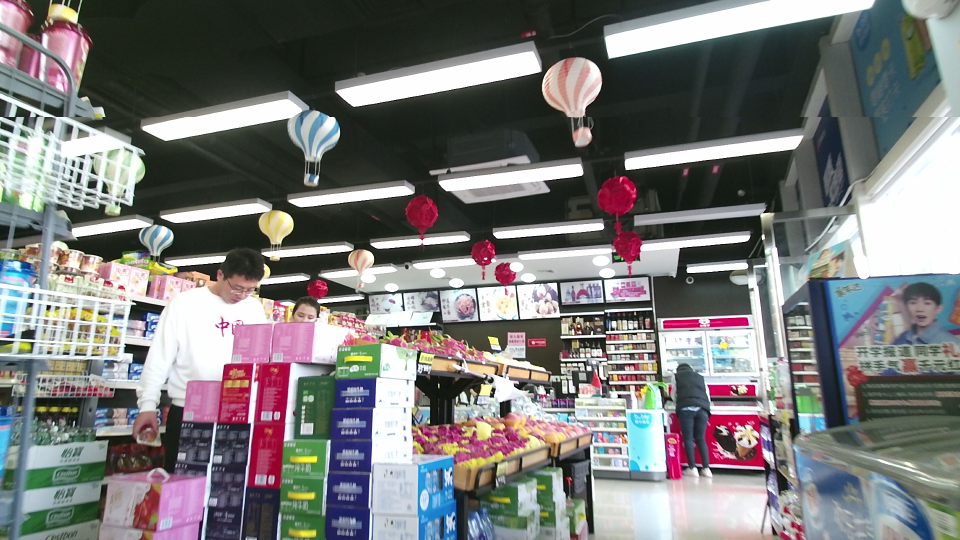
\includegraphics[width=.32\linewidth]{figures/extended-thud_dense_test50-6-rgb.png}\hfill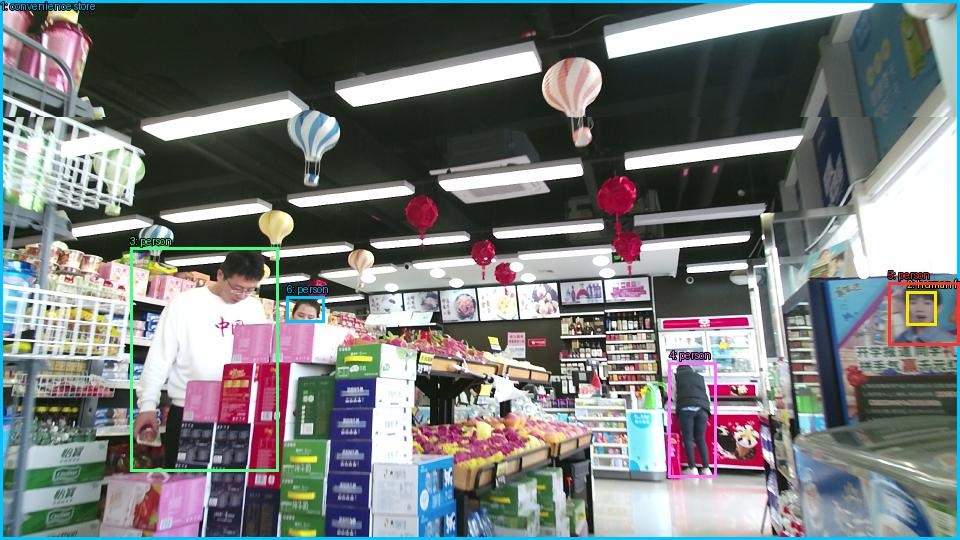
\includegraphics[width=.32\linewidth]{figures/extended-thud_dense_test50-6-od.jpg}\hfill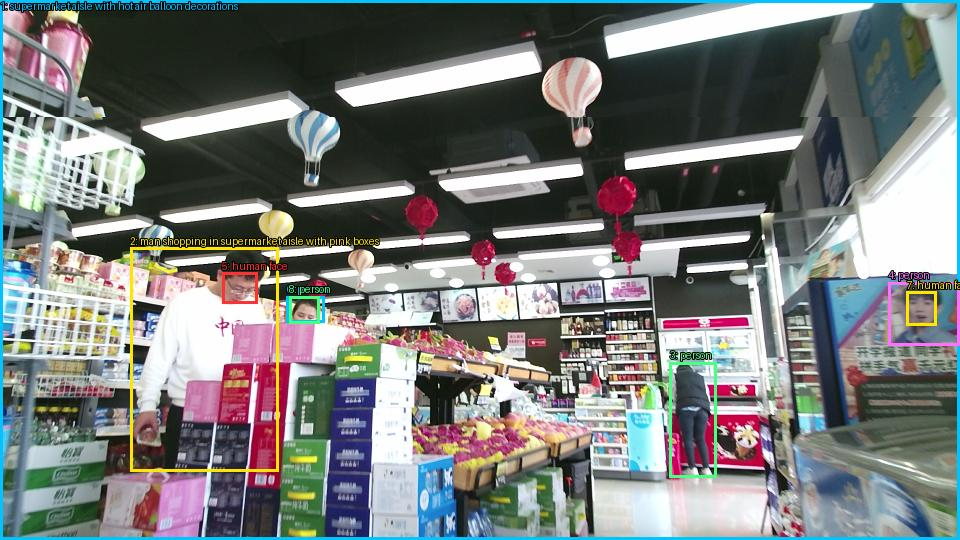
\includegraphics[width=.32\linewidth]{figures/extended-thud_dense_test50-6-dense.jpg}\\{\scriptsize Levo: RGB; sredina: OD; desno: DENSE\_REGION\_CAPTION. Okvirji so napovedi, ne reference.}\end{center}
\begin{center}\small\begin{tabular}{p{3.2cm}p{1.1cm}p{11cm}}\toprule
Model & Zapis & Dejanski izsek / napaka \\ \midrule
NVILA-8B FP16 & error & A grocery store interior with various products and decorations. The ceiling is adorned with colorful hot air balloon-shaped lights, and there are shelves stocked with items like beverages, snacks, and fruits. A... \\
Florence-2-large FP16 & ok & The image shows the interior of a supermarket aisle with a variety of items on display. The aisle is filled with shelves stocked with different types of food and drinks. On the left side of the image, there is ... \\
Qwen BF16 (staro) & ok & An indoor retail environment with black ceilings and fluorescent lighting. Decorative hot air balloons and red lanterns hang from the ceiling. Shelves on the left hold packaged goods, while a central display fe... \\
Qwen Q4 (staro) & ok & An indoor retail environment with black ceiling panels and long rectangular fluorescent lights. Decorative hot air balloons in blue/white, yellow, and red/white patterns hang from the ceiling along with red pap... \\
Gemma Q4 (staro) & error & The photograph depicts a brightly lit supermarket interior. Several shelves stocked with various products are visible, including fruit, beverages, and packaged goods. A customer, wearing a white shirt, is stand... \\
\bottomrule\end{tabular}\end{center}
\textbf{Lastni delni vizualni pregled:} Florence OD okvirji zajamejo velikega moškega levo, osebo zadaj desno in delno zakrito glavo za moškim; to je uporaben uspeh lokalizacije. Kot person in human face označi tudi obraz na plakatu desno, kar ni nova fizična oseba v prostoru. Dense dvakrat vrne skoraj isti okvir delno zakrite glave; podregije/ponovitve ostanejo ločene. NVILA omenja shopping basket pri moškem, ki ga na sliki ne morem potrditi; trditev ostane modelova. Prejšnji Qwen BF16 je v bogatem opisu ločil tri osebe. To ni celotna referenca detekcije.
\subsection*{Dejanske besedilne presoje novih opisov}\begin{center}\small\begin{tabular}{p{1.6cm}p{4.2cm}p{1.8cm}p{7.6cm}}\toprule
Opis & Dobesedni objekt & Razred & Modelov razlog \\ \midrule
nvila & man in white shirt & movable & Person is not part of the robot map structure. \\
nvila & shelf with beverages and snacks & movable & Shelf appears freestanding and can be repositioned. \\
florence & convenience store & movable & Convenience store is a building, not a robot map object. \\
florence & human face & uncertain & Human face cannot be classified as fixed or movable structure. \\
\bottomrule\end{tabular}\end{center}
Različna imena niso potrjeno iste instance. To so modelove presoje; brez referenc stabilnosti jih ne štejemo kot accuracy.

\newpage
\section*{Dejanski primeri: fotografija in Florence regije}\subsection*{agtea / indeks 1}
\begin{center}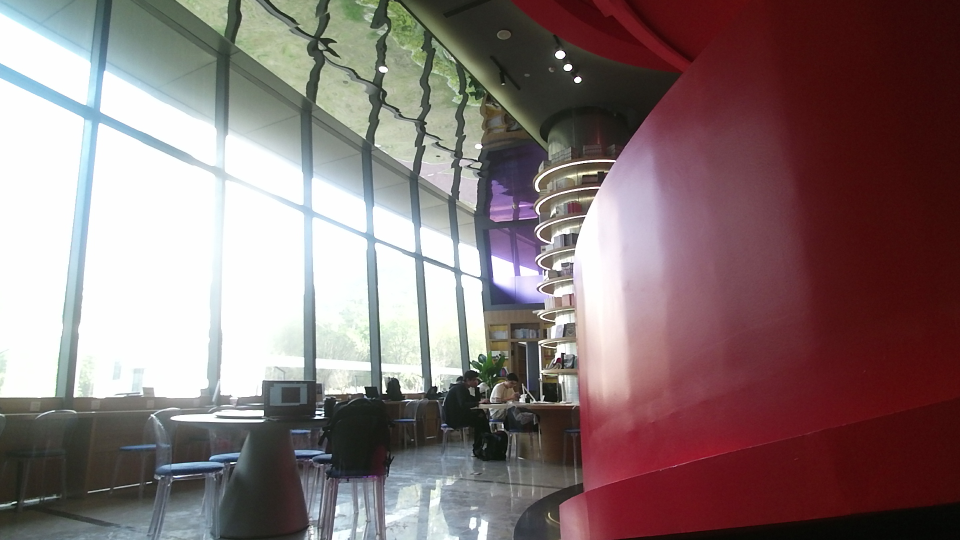
\includegraphics[width=.32\linewidth]{figures/extended-thud_agtea_test50-1-rgb.png}\hfill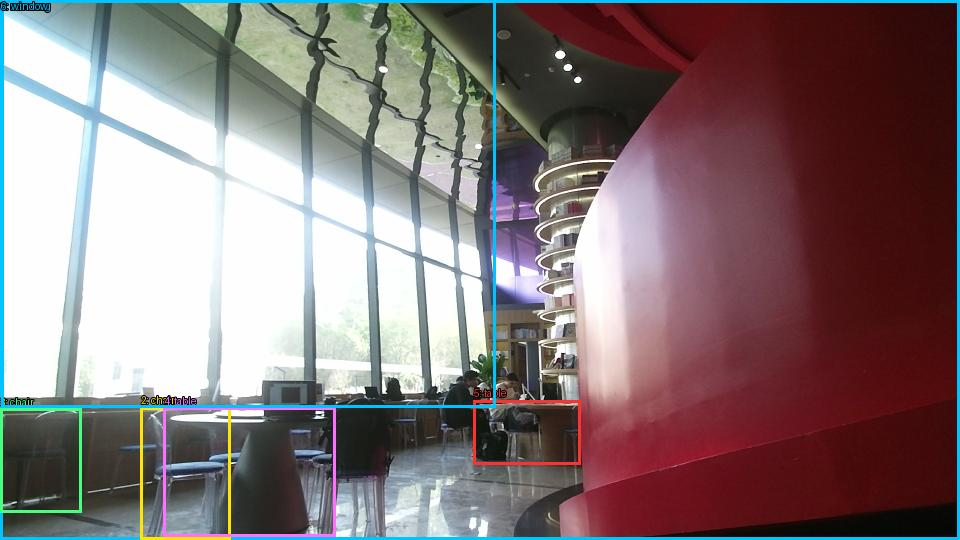
\includegraphics[width=.32\linewidth]{figures/extended-thud_agtea_test50-1-od.jpg}\hfill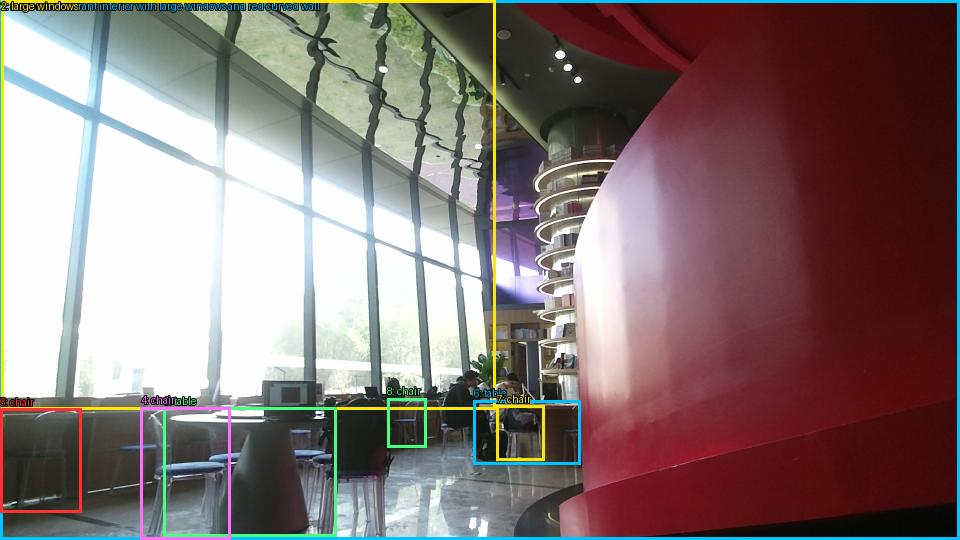
\includegraphics[width=.32\linewidth]{figures/extended-thud_agtea_test50-1-dense.jpg}\\{\scriptsize Levo: RGB; sredina: OD; desno: DENSE\_REGION\_CAPTION. Okvirji so napovedi, ne reference.}\end{center}
\begin{center}\small\begin{tabular}{p{3.2cm}p{1.1cm}p{11cm}}\toprule
Model & Zapis & Dejanski izsek / napaka \\ \midrule
NVILA-8B FP16 & error & A modern cafe interior with large windows, a red wall, and a spiral bookshelf. There are tables with laptops and chairs, and people sitting at the tables. The floor is shiny marble, and there's a green plant ha... \\
Florence-2-large FP16 & ok & The image shows the interior of a modern restaurant or cafe. The room has a large window on the left side, allowing natural light to enter the space. The floor is made of marble tiles, and there are several tab... \\
Qwen BF16 (staro) & ok & An indoor space with large windows on the left letting in bright light. A tall red curved structure dominates the right foreground. In the background, there are tables and chairs where people are seated. A spir... \\
Qwen Q4 (staro) & ok & An indoor space with large windows on the left letting in bright light. A tall red curved structure dominates the right foreground. In the background, there are tables and chairs where people are seated. A spir... \\
Gemma Q4 (staro) & ok & The photograph depicts a brightly lit interior space with large windows offering a view of trees and foliage. A curved, red wall dominates the right side of the frame, while a tall window extends across the maj... \\
\bottomrule\end{tabular}\end{center}
\textbf{Lastni delni vizualni pregled:} Florence pravilno postavi veliko okno levo in vrne pregledne okvirje več stolov ter miz. Splošni opis pa dodaja spiral staircase in enjoying their meals; iz te fotografije teh trditev ne morem potrditi. Viden je krožni element s knjigami; opis stopnišča zahteva dodatni dokaz. Okvirji se lahko prekrivajo čez zakrite stole/mize in niso dokaz pravilnih stikov ali materialov. Stari Qwen BF16 je stole napačno opisal kot transparent plastic. Delni vizualni pregled. NVILA pravilno poimenuje spiral bookshelf, vendar doda green plant hanging from ceiling, ki je na tej fotografiji ne morem potrditi. Material marble ostane nepotrjena modelova trditev; odsev tal ga ne dokazuje.
\subsection*{Dejanske besedilne presoje novih opisov}\begin{center}\small\begin{tabular}{p{1.6cm}p{4.2cm}p{1.8cm}p{7.6cm}}\toprule
Opis & Dobesedni objekt & Razred & Modelov razlog \\ \midrule
nvila & large window & fixed & Large structural window panel integrated into building frame. \\
nvila & red wall & fixed & Integral part of the building's permanent wall structure. \\
florence & building & fixed & Building structure requires dismantling to relocate. \\
florence & chair & movable & Chair can be carried or repositioned in normal use. \\
\bottomrule\end{tabular}\end{center}
Različna imena niso potrjeno iste instance. To so modelove presoje; brez referenc stabilnosti jih ne štejemo kot accuracy.

\newpage
\section*{Dejanski primeri: fotografija in Florence regije}\subsection*{agtea / indeks 6}
\begin{center}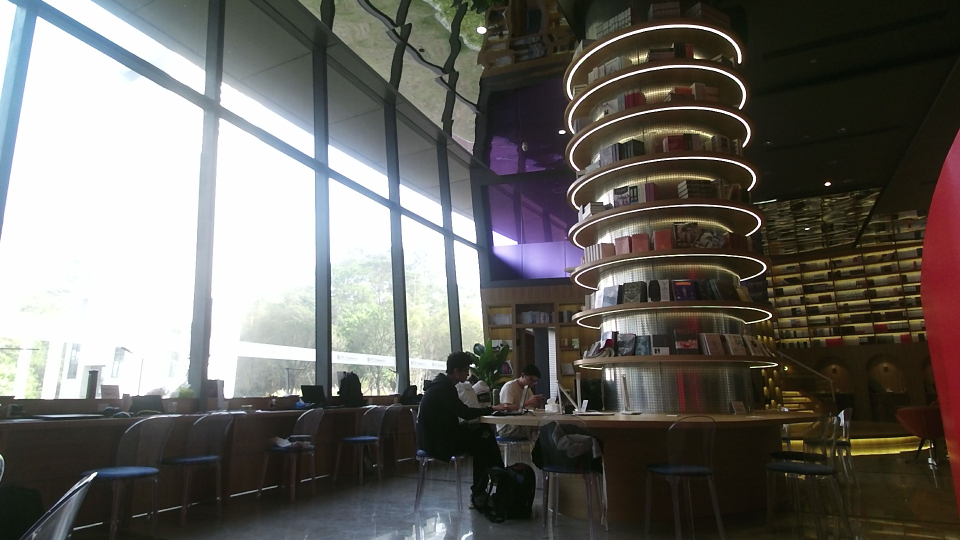
\includegraphics[width=.32\linewidth]{figures/extended-thud_agtea_test50-6-rgb.png}\hfill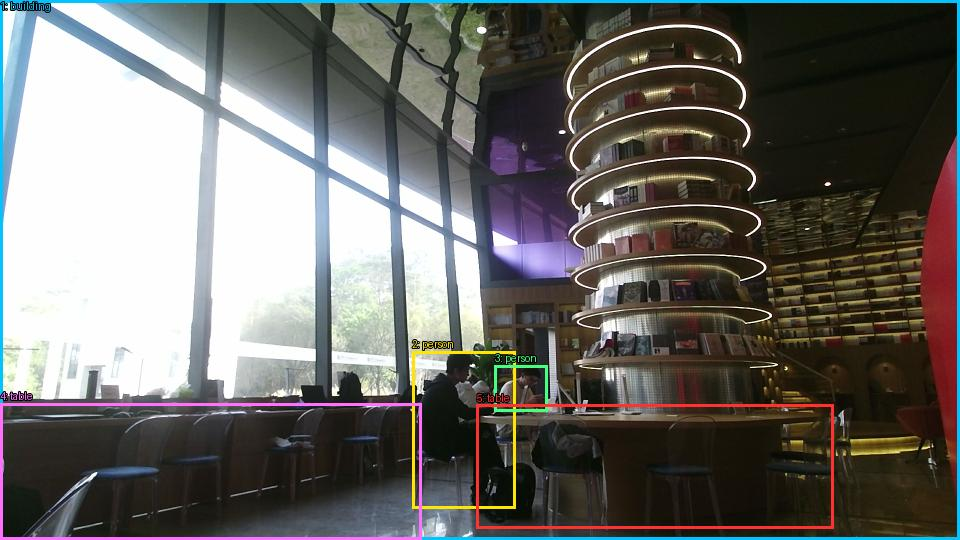
\includegraphics[width=.32\linewidth]{figures/extended-thud_agtea_test50-6-od.jpg}\hfill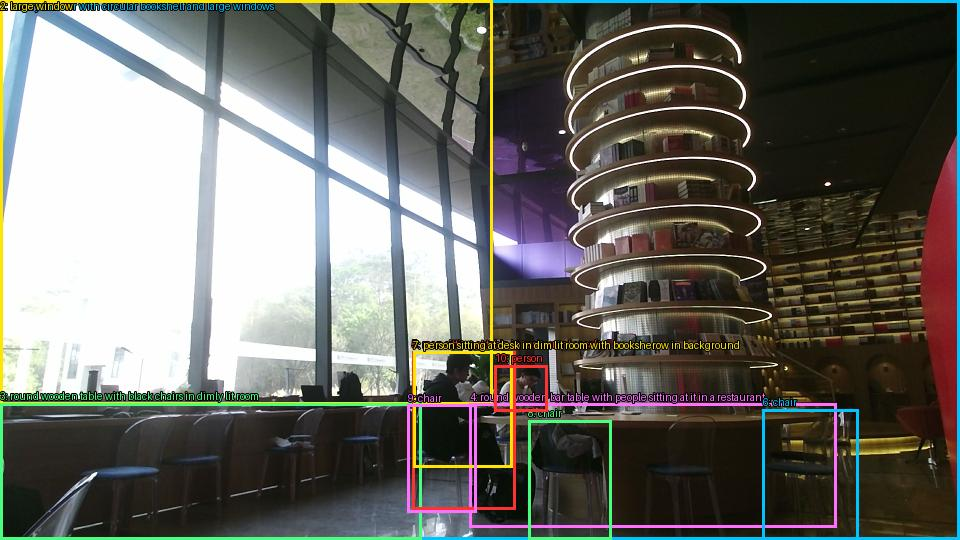
\includegraphics[width=.32\linewidth]{figures/extended-thud_agtea_test50-6-dense.jpg}\\{\scriptsize Levo: RGB; sredina: OD; desno: DENSE\_REGION\_CAPTION. Okvirji so napovedi, ne reference.}\end{center}
\begin{center}\small\begin{tabular}{p{3.2cm}p{1.1cm}p{11cm}}\toprule
Model & Zapis & Dejanski izsek / napaka \\ \midrule
NVILA-8B FP16 & error & A modern library interior with a large circular bookshelf and tall windows. The room is well-lit, with natural light coming through the windows and artificial lighting from the bookshelf. There are several peop... \\
Florence-2-large FP16 & ok & The image shows the interior of a modern library with a large window on the left side. The window offers a view of the trees and buildings outside. On the right side of the image, there is a tall spiral stairca... \\
Qwen BF16 (staro) & error & An indoor space with large windows on the left letting in bright light. A tall, spiral bookshelf structure stands centrally, illuminated by rings of lights. People sit at tables nearby. The floor is reflective. \\
Qwen Q4 (staro) & ok & An indoor public space with large windows on the left letting in bright daylight. A tall, spiral bookshelf structure stands centrally, illuminated by rings of light. People are seated at tables near the window ... \\
Gemma Q4 (staro) & ok & The photograph depicts a brightly lit interior space, likely a library or bookstore, with a large window providing natural light. A prominent feature is a tall, circular bookshelf illuminated by internal lights... \\
\bottomrule\end{tabular}\end{center}
\textbf{Lastni delni vizualni pregled:} Florence dense pravilno poimenuje circular bookshelf, vrne regije dveh oseb levo od krožnega knjižnega elementa in več stolov. Splošni caption isti element napačno razlaga kot tall spiral staircase with bookshelves on both sides; več ravni police samo po sebi ni vidno stopnišče. Regionalne fraze wood/black chairs in restaurant niso zanesljiva potrditev materiala, barve ali tipa prostora; vidni so tudi modri sedeži in kovinski okvirji. Razlika med caption in dense je konkreten primer nestrinjanja nalog istega modela. Delni vizualni pregled. NVILA pravilno prepozna circular bookshelf in obodne luči, nato trdi visible mounting hardware/support beams in securely mounted to the floor; teh pritrditev ne morem potrditi. Isti odgovor hkrati pravi, da ni vidno, ali je polica pritrjena na tla ali prostostoječa. To notranje protislovje ostane v surovem besedilu za presojo.
\subsection*{Dejanske besedilne presoje novih opisov}\begin{center}\small\begin{tabular}{p{1.6cm}p{4.2cm}p{1.8cm}p{7.6cm}}\toprule
Opis & Dobesedni objekt & Razred & Modelov razlog \\ \midrule
nvila & circular bookshelf & uncertain & Evidence of mounting conflicts with description of functional furniture. \\
florence & building & movable & Building exterior or large structure, typically movable in map context. \\
florence & person & movable & Person is a biological entity, inherently movable. \\
\bottomrule\end{tabular}\end{center}
Različna imena niso potrjeno iste instance. To so modelove presoje; brez referenc stabilnosti jih ne štejemo kot accuracy.

\newpage
\section*{Sklep nadaljevanja in ponovljivost}
\subsection*{Konkretne ohranjene napake in rešitve}
Florence se je po 37 shranjenih slikah končal s procesnim izhodom 132 (SIGILL), brez Python izjeme. Nadaljevanje z vključeno sledjo faulthandler je dokončalo vseh 100 slik brez ponovitve že shranjenih odgovorov. Vzrok ni potrjen; ponovnega zagona ne predstavljamo kot dokazanega popravka odvisnosti. En dense izhod agtea, indeks 24, vsebuje obrnjen okvir [0,48; 31,05; 87,84; 0,27]. Celoten izhod ostane zavrnjen; ločen rdeč diagnostični izris ohrani prvotni vrstni red koordinat. Ne obrnemo ga v veljaven okvir in ne vključimo v ujemanje.

NVILA začetno ogrevanje in merjeni pilot z repetition\_penalty=1,0 oba dosežeta 8192 tokenov s ponavljanjem JSON. Pri 1,05 je prvi merjeni odgovor kratek, vendar se zanke pri nekaterih drugih slikah še pojavijo. Pogoste so tudi dodatno besedilo za JSON, manjkajoča polja in napačna sintaksa. To so izmerjene omejitve formata modela, ne več nedelujoč GPU. Celotni odgovori, tudi zavrnitve in odmevi navodil, ostanejo shranjeni. Besedilni transport za razvrščanje ne spremeni teh rezultatov validacije.

Po uspešnem zaključku NVILA kontejnerja (izhod 0, vseh 100 odgovorov) je lupinski zaganjalnik javil sintaktično napako. Datoteka je bila med izvajanjem urejena; to je verjetna, ne dokazana razlaga. Razvrščanje je bilo nato uspešno izvedeno ločeno. Novi zaganjalnik najprej razčleni celotno funkcijo. GPU dnevnik ima 374 veljavnih vzorcev in poškodovan zaključek 125 ničelnih bajtov po meritvah; izvirnik ostane shranjen, veljavne vrstice so izvožene ločeno. Vrhovi VRAM v tabelah izhajajo iz inferenčnih zapisov.

Obe zahtevani novi okolji sta pripravljeni za dejansko slikovno inferenco na RTX 5090. Priročnost formata, uspešen GPU zagon in veljavnost izhoda so ločene ugotovitve od vizualne kakovosti. Primerjava vključuje tudi zavrnjene odgovore in razliko med splošnim opisom, detekcijo in regionalnim opisovanjem. Celoten pregled istih 20 fotografij z vsemi starimi/novimi odgovori, referencami in presojami je lokalno v manual-review.html. Preglednica 40 novih model/slika vrstic ostane pending; štirje prikazani primeri so samo delni pregled, ne izmišljena celotna referenca.

Surovi novi izhodi: \texttt{results/thud-extended/}; tam so originalni tokeni, razčlenjeni odgovori, konfiguracije, izvorne kode/SHA, pripete uteži, Docker dnevniki, diagnostika in vsi izrisi. Obstoječi odgovori so preverjeni proti indeksu SHA256 pred nadaljevanjem. Git vsebuje kodo, Dockerfile, navodila, agregate, izbrane slike, PDF in LaTeX. Točne revizije modelov in dejanski tipi parametrov so v extended-model-metadata.json in manifestih; dolgi izhodi ostanejo lokalno.
Celotna zbirka: 69 testov, 9.065 s, vsi uspešni.
\begin{verbatim}
bash scripts/thud_extended.sh prepare
bash scripts/thud_extended.sh nvila 1
bash scripts/thud_extended.sh nvila 100
bash scripts/thud_extended.sh florence 1
bash scripts/thud_extended.sh florence 100
bash scripts/thud_extended.sh reason
bash scripts/thud_extended.sh report
python3 -m unittest discover -s tests -v
\end{verbatim}
Izvajalnika zahtevata GPU brez CPU nadomestila. Vsako novo nalaganje fizično ogrejeta; že shranjene merjene odgovore (tudi napake) nadaljujeta brez ponovitev. Spremenjeni vhodi/nastavitve zahtevajo ločen poskus. Za vseobsegajoč zagon je na voljo all. Samo faza report ne izvaja inferenc. Neposredni NVILA izvajalnik ne odpira slikovnega API, zato ne trdimo, da stari strežnik deluje.

Naslednji korak naj bo ročni pregled pokritosti posameznih instanc in dejanskih podpor/stikov na istih 20 slikah. Namenske naloge Florence ne zagotovijo ustrezne granularnosti samo s tem, da vrnejo okvirje; NVILA ne postane najboljši model samo zaradi več parametrov ali več besed. Izbira mora upoštevati kakovost in napake skupaj s stroškom. Stabilnosti ne moremo potrditi z eno fotografijo.
\vfill{\footnotesize Uradni viri: \href{https://huggingface.co/Efficient-Large-Model/NVILA-8B}{NVILA-8B}, \href{https://github.com/NVlabs/VILA/tree/57ecbfb904b99b563db69ef7916f6390eecea516}{pripeta NVIDIA VILA koda}, \href{https://huggingface.co/microsoft/Florence-2-large}{Florence model in izvirne naloge}, \href{https://pytorch.org/get-started/previous-versions/}{PyTorch CUDA različice}. Preverjeno 21. 10. 2026.}
